\documentclass[11pt,a4paper]{article}
\usepackage[utf8]{inputenc}
\usepackage{graphicx}

\usepackage{hyperref}

\usepackage{fancyhdr}
\pagestyle{fancy}

% \textheight=22cm
% \textwidth=14.945cm
% \topmargin=0.5cm
\headheight=14pt
% \headsep=0cm
% \oddsidemargin=0.5cm
% \evensidemargin=0.5cm
% \columnsep=0.8cm
% \renewcommand{\baselinestretch}{1.3}

\begin{document}

% Todo: change to tktl layout
\begin{titlepage}

  \begin{flushleft}
  \large
  \noindent YaJTris - Yet another Java Tetris \\
  Jussi Mäki \\
  Rälssintie 16 D 40 \\
  00720 Helsinki \\
  Email: \href{mailto:joamaki@gmail.com}{joamaki@gmail.com} \\
  \end{flushleft}

  \begin{center} \sloppy
    \vfill

    \huge \textbf{Implementation document} \vfill

    \vspace{3mm}
  \end{center}

  \begin{flushright}
    \large
    University of Helsinki \\
    Computer Science department \\
    Programming project (Java)\\
    Instructor Mika Holmström

    Helsinki \today
    % \number\day .\number\month .\number\year
  \end{flushright}

\end{titlepage}


% Hide page number in toc
\thispagestyle{empty}

\tableofcontents

\setcounter{page}{1}
\newpage

\section {User manual}

\subsection {Introduction}

YaJTris is a clone of the still popular Russian computer game \href{http://en.wikipedia.org/wiki/Tetris}{Tetris} by Alexey Pajitnov in 1985.
YaJTris is written in the Java programming language and is thus portable to a wide range of systems that are supported
by the Java Runtime Environment (JRE).

\subsection {Installation}

YaJTris is distributed in a zip-package. The package contains sources, documentation and a
ready-to-run jar file. YaJTris has been precompiled with Sun Java version 1.5.0 (Java 5 SE) and thus
should run on all runtimes from 1.5 and up. It may work with non-Sun implementations but it has only been tested
with Sun's implementation.

To install YaJTris just extract the package to desired location.

\subsection {Running}

The distribution contains scripts to start YaJTris.

For Windows platforms a script yajtris.bat
is provided and double clicking it on explorer should start the game.

For UNIX platforms there's yajtris.sh. First make sure that the script is executable with command
``chmod +x yajtris''. After that you can start YaJTris with command ``./yajtris.sh''. If this fails
make sure that 'java' program is found in path or that JAVA\_HOME is set to the location of
your Java installation. Refer to Sun's Java installation documentation if in trouble.

You can also try starting YaJTris manually with command: 'java -jar yatris.jar'.

\subsection {Playing}

YaJTris is played on a board of 10x20 squares. The objective is to place tetrominoes
(7 distinct pieces made from 4 squares) one at a time on the board into lines which, when completed, are
cleared from the board. The pieces drop from the upper edge of the board at a steady rate determined by the current level.
These pieces never run out, but the space on board will so make sure you keep the board clean and organized.
The game ends when a piece no longer can drop freely from the upper edge of the board.

As most tetris clones YaJTris makes use of the cursor keys to move the tetromino. Use
the LEFT and RIGHT keys to move the piece left and right respectively. Use the 'UP' key to
rotate the piece and 'DOWN' key to move the piece down faster. To drop the piece press 'SPACE'.

To make things more interesting the player is awarded points for every cleared line. These points
are determined by the current level and the number of lines cleared at a time.

The game partly implements the scoring system used in the Nintendo Tetris as specified at \\
\href{http://www.tetrisconcept.com/wiki/index.php?title=Scoring\#Original_Nintendo_scoring_system}{Original nintendo scoring}.
The scoring scheme is as follows: for one line you score 40*(level+1) points, for two lines 100*(level+1), for three lines 300*(level+1) and
for four lines 1200*(level+1).

When the game ends and you make it to the top ten you'll be prompted for initials (3 characters).

To exit the game press 'ESCAPE' to end the current game. And press 'ESCAPE' again
when the screen says ``Press escape to exit''. You may need to input initials
to be entered into the high scores list before this.

Word of warning: The game is known to be very addictive so make sure you don't have anything urgent to do before
you start playing!

\begin{center}
  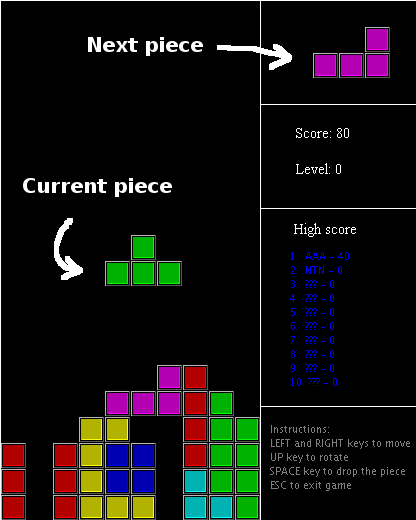
\includegraphics[scale=0.5]{screenshot.png}
\end{center}

\subsection {Compiling}

If you wish to recompile YaJTris there's GNU Makefiles provided to help with the compilation.
On a system with GNU make run 'make' in the root of the YaJTris distribution.

On Windows systems without GNU make you can compile YaJTris manually with 'javac'. Change to the
source directory and run 'javac Game.java'. This should produce the necessary java .class files to
start the game or produce a .jar file. To create a jar-file run the command:
'jar cvfm yajtris.jar manifest *.class'.


\section {Program structure and internals}
\subsection {Overview}

I strived to keep the design as simple as possible and not overdo it with
overly fancy object-orientated design. There are only 4 classes: the main class,
a board class, a tetromino class and a high scores class.
All the core game functionality is in the main class. The module is still sufficently compact to not
 warrant splitting up the functionality in to discrete classes.
The board class presents a n-by-n board of squares. It is used to draw fallen
tetrominoes and also to provide a way for the tetromino class to draw itself
thus limiting the drawing of squares to the board class as well as limiting the
duplication of board coordinates and size.
The tetromino class presents the current tetromino in play. It provides methods
for moving and rotating the piece. It mostly interfaces with the board class
to draw itself and to check for collisions with the board. When the tetromino is
``retired'' it is placed on the board.
The high scores class allows for saving, loading and displaying of high scores.

The largest (although not in any way difficult) to figure out was implementing
the rotation of the tetromino. The first method I tried was representing the block
in a 4x4 array and rotating the array in order to rotate the block. This however caused
the block to move off-center when rotated. Solution was to increase the size
of the array to 5x5. However the resulting rotations are not completely similar
to those found in some other tetris games, but the game play was minorly effected by this
and the code is much simpler.

The gist of the documentation is available in javadoc generated HTML-pages in the
javadoc/ directory.

\subsection {Class diagram}

\vspace{3mm}
\begin{center}
  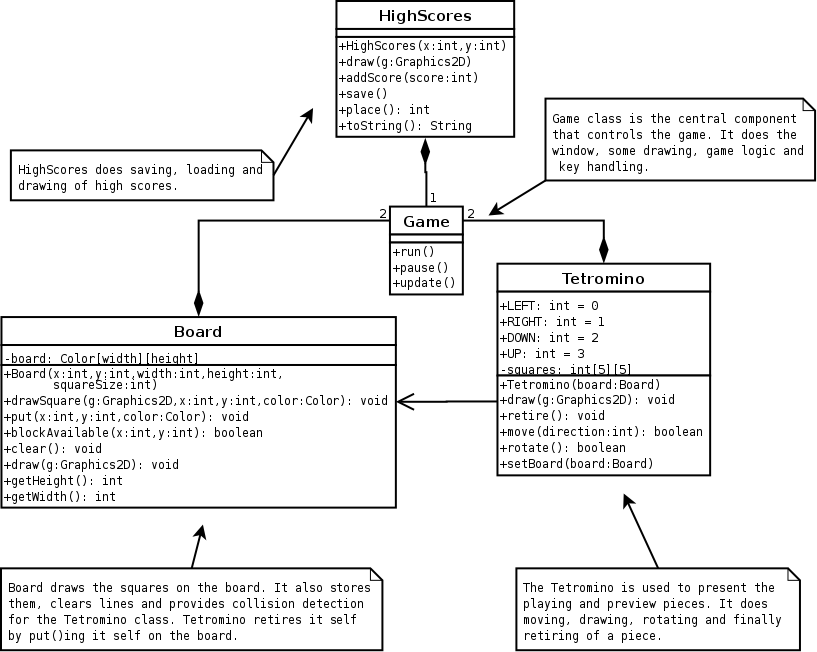
\includegraphics[scale=0.3]{class_diagram.png}
\end{center}

\subsection {Class descriptions}

The detailed class descriptions are available in javadoc.

\newpage
\subsection {Class interactions}

\begin{itemize}
\item Game logic
  \begin{center}
    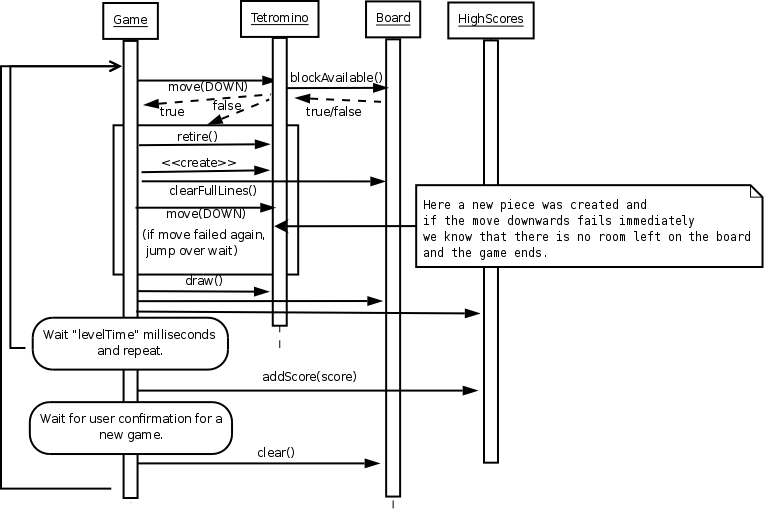
\includegraphics[scale=0.30]{seq_game.png}
  \end{center}

\item Rotating and moving a tetromino
  \begin{center}
    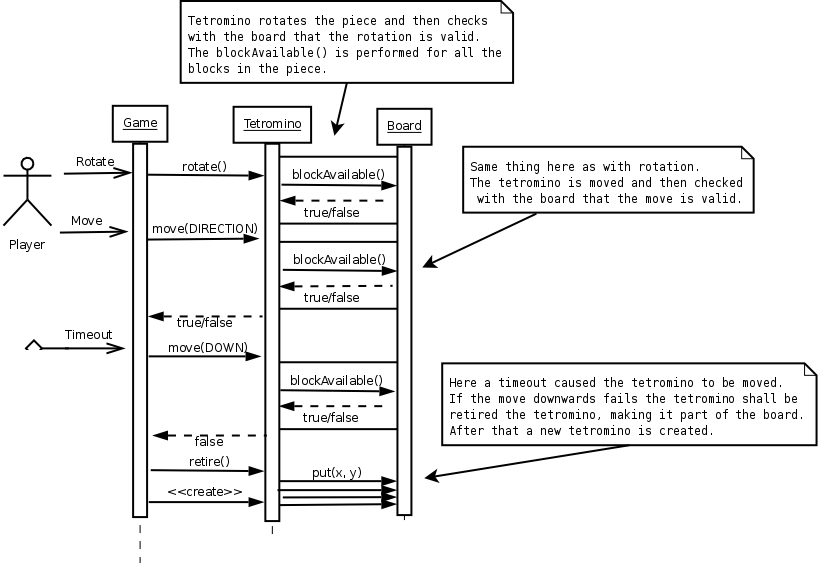
\includegraphics[scale=0.26]{seq_tetro.png}
  \end{center}
\end{itemize}

\subsection {Improvement ideas}

To enhance the game play sounds and music could be added to the game.
Graphics could also be enhanced. Instead of relaying on Java2D to draw
the pieces, board and text, bitmaps could be used instead to gain a
more arcade-like look for the game.

Code could be refactored. Especially the main class might need
refactoring if more functionality were added. The board and tetromino
interactions might need rethinking. Graphics-related code could be separated
from the board and tetromino handling although it'd probably only serve to make the
program more complicated without giving much in return.

Major optimizations are possible to the board drawing code. Currently
no algorithm for determining what parts to redraw is used instead everything
on the screen is redrawn.

Unit tests do not cover enough of the code. The Game class would need
refactoring in order for it to be unit testable.

\section {Testing}
% todo: fix this section to correspond to instructions at
% http://www.cs.helsinki.fi/u/jnenonen/alabra/toteutusdoc.html

\subsection {Unit tests}

The unit tests test individual modules. The tests are specified in Java and are run
with command 'make test'. Some of the tests may need a human supervisor.

\begin{itemize}
\item UT-TC1: Test1.java: Board and Tetromino test
  This test program was created for testing the board and tetromino
  classes. The program creates a board and several tetrominoes.
  It moves and rotates each of the tetrominoes randomly around the
  board. This tests that moving, rotating and drawing
  tetrominoes on the board works.

  This test is not meaningful unless an observer sees that the rotations and moves
  are correctly displayed in the window.

\item UT-TC2: Test2.java: High scores test
  This test program tests the HighScores class. It creates, saves
  and loads scores. It does not test drawing of scores however.
\end{itemize}

Both the unit tests passed on tests conducted on 24.2.2008.

\subsection {System tests}

The system tests test the system functionality. The tests are executed manually according to the
following test cases.

As a preparation for the tests remove the high scores file 'yajtris.dat'.

\begin{itemize}
  \item ST-TC1: Starting the game and getting pass the intro-animation
    Start application as specified in the user manual.

The intro-animation should come up.
    A group of moving and rotating tetrominoes should appear with a text hovering over them.
    Press a key to start the game. The game screen as shown in user manual should appear.

    Expected outcome: The game starts and the user is presented with an intro-animation that is passed when user presses any key.

    Test status as executed on 24.2.2008: Test passed.

  \item ST-TC2: Rotation and moving
    After ST-TC1 you should be in the game. Test rotation of the current piece using the 'UP' key. Test all
    possible rotations for the piece. Then test moving using the 'LEFT' and 'RIGHT' keys. Move the piece to the leftmost
    wall with the 'LEFT' key. Then test rotation with the 'UP' key. The piece may or may not rotate depending on the type of piece.
    Then do the same thing in the rightmost corner using the 'RIGHT' key. Now repeat the test with all the seven pieces. If needed
    you may start a new game by pressing the 'ESC' key and following on screen instructions.

    After this test that the 'SPACE' key drops the piece.

    Notes: This test does not cover all the corner cases, but only that the simplest rotations and moves work. This test
           requires knowledge of tetris in order to deduct correct outcome.

    Expected outcome: Piece moves and rotates as expected.

    Test status as executed on 24.2.2008: Test passed.

  \item ST-TC3: Clearing a line
    Construct a line by dropping the pieces to fill a horizontal line.

    Expected outcome: The squares along the line disappear from the board and the lines above it get shifted down by one square.

    Test status as executed on 24.2.2008: Test passed.

  \item ST-TC4: Game over and high scores.
    Test the game over situation by dropping the pieces until the top of the board is reached. The game should end and you should
    see a high score input screen. Enter AAA and wait for the game over screen to appear. Press enter to start a new game. The
    AAA entry should be visible in the high score list on the right side of the screen.

    Now abort the current game by pressing Escape. You should be asked for high score initials input again for which you can enter
    AAA again. On the game over screen press Escape again to exit the game. After the game has exited restart it and start a new
    game. Check the high scores list again for the inputted initials.

    Expected outcome: The input of high scores initials worked, starting a new game from the game over screen works and exiting
                      the application from the game over screen works. After starting the game from scratch the saved high scores
                      were loaded and appeared on the high score list.

    Test status as executed on 24.2.2008: Test passed.

\end{itemize}

\end{document}
